\chapter{Light and Color}


\section*{LEARNING OUTCOMES}
{
\begin{center}
\fcolorbox{black}{shadecolor}{%

    \parbox{0.95\textwidth}
    {%
        \small
        {
        \begin{itemize}[leftmargin=*]\itemsep0em
            \item How does light travel?
            \item What causes shadows?
            \item What are the different types of media (transparent, translucent, opaque)? How does light travel through them?

            \end{itemize}
        }
    }%
}
\end{center}
}

\section*{DEMONSTRATIONS}
\section*{1. Formation of Shadows}
Interfacing a light sensor with Arduino to show that shadows are formed by an absence of light. Th intensity of light is recorded by the sensors and the measurements are shown graphically on the screen.

\begin{table}[H]
    \centering
    \begin{tabular}{|c|l|c|}\hline
     \textbf{\#} & \textbf{Components} &  \textbf{Amount}\\\hline
    1 & LDR                     & 1\\\hline
    2 & 1 k$\Omega$ resistor    & 1\\\hline
    3 & Torch                   & 1\\ \hline
    4 & Arduino UNO             & 1 \\\hline
    5 & Breadboard              & 1 \\\hline
    6 & Connecting wires        & - \\\hline
    \end{tabular}
\end{table}

\subsection*{Connections}
\begin{enumerate}[leftmargin=*]
    \item Connect the 5V pin and GND pin of the Arduino board on the breadboard. 
    \item Connect one terminal of the LDR to 5V. 
    \item Connect one terminal of the 1 k$\Omega$ resistor to the free terminal of the LDR. Connect its other terminal to GND.
    \item Connect the junction of the LDR and the resistor to pin A0 of Arduino.
\end{enumerate}

Fig. \ref{fig:shadows} shows the circuit diagram of this experiment.

\begin{figure}[H]
    \centering
    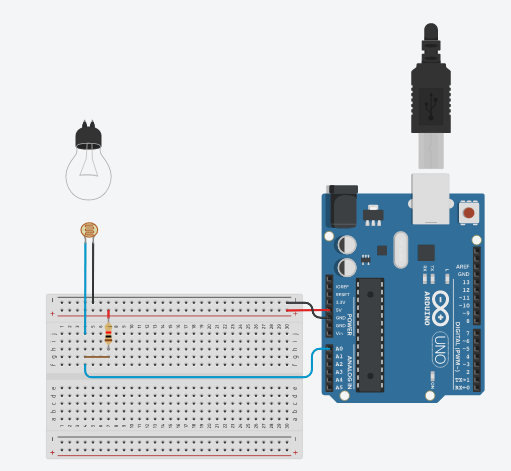
\includegraphics[scale=0.5]{Figures/shadow.png}
    \caption{Circuit diagram}
    \label{fig:shadows}
\end{figure}

\subsection*{Procedure}

\begin{enumerate}[leftmargin=*]
    \item Copy lst. \ref{lst:shadows} to a new Arduino sketchbook. Upload the code to your Arduino board. Also open the Serial Monitor.
    \item Shine a bright light on the LDR. Observe the change in the readings taken by Arduino.
    \item Block the light using cardboard so that it does not reach the LDR. Observe the change in the readings taken by Arduino. Do you see a shadow? Does Arduino indicate the same?
\end{enumerate}
\begin{lstlisting}[language=Arduino, numbers=none, caption={Arduino code for measuring the intensity of light measured by LDR}, captionpos=b, label={lst:shadows}]

int shadow=A0;  

void setup() 
{
  // put your setup code here, to run once:
  pinMode(shadow, INPUT);    // A0 is declared an input peripheral
  Serial.begin(9600);
}

void loop() 
{
  // put your main code here, to run repeatedly:
  
  int intensity = analogRead(shadow);    
  // The intensity of light on the LDR is recorded
  
  Serial.print(intensity);          
  // The light intensity is printed either on Serial Monitor or on Serial Plotter
  
    if (intensity>100)
        Serial.println("\t light");
    else
        Serial.println("\t shadow");
        
    delay(50);                      //Add a delay of 50 ms
}

\end{lstlisting}
% ---------------------------------------------------
\section*{2. Formation of Colors from Primary Colors of Light}
Change the intensity of red, blue and green light in RGB LED to show the formation of different colors.

For this experiment, you'll need:

\begin{table}[H]
    \centering
    \begin{tabular}{|c|l|c|}\hline
     \textbf{\#} & \textbf{Components}  &  \textbf{Amount}\\\hline
    1 & 1 k$\Omega$ potentiometers      & 3\\\hline
    2 & 470 $\Omega$ resistors          & 6\\\hline
    3 & RGB LED                         & 1\\\hline
    4 & Red LED                         & 1\\ \hline
    5 & Blue LED                        & 1\\\hline
    6 & Green LED                       & 1\\\hline
    7 & Arduino UNO                     & 1 \\\hline
    8 & Breadboard                      & 1 \\\hline
    9 & Connecting wires                & - \\\hline
    \end{tabular}
\end{table}

\subsection*{Connections}
\begin{enumerate}[leftmargin=*]
    \item Connect the 5V pin and GND pin of the Arduino board on the breadboard. 
    \item Mount the potentiometers on the breadboard. Connect their left terminal to 5V and their right terminal to GND. 
    \item Connect the middle terminal of each potentiometer to 470 $\Omega$ resistors. 
    \item Connect the free terminal of each resistor with the anode of red, green and blue LEDs respectively. 
    \item Connect the cathode of each LED with GND.
    \item Connect the terminal at the junction of the potentiometer and the resistors to pins A$0$, A$1$ and A$2$ respectively.
    \item Connect the cathode of the RGB LED to GND.
    \item Connect the anodes of RGB LEDs to 470 $\Omega$ resistors.
    \item Connect the free terminals of the resistors controlling red, green, and blue LED of RGB LED to pins 9, 10 and 11 of Arduino respectively. 
\end{enumerate}

\begin{figure}[H]
    \centering
    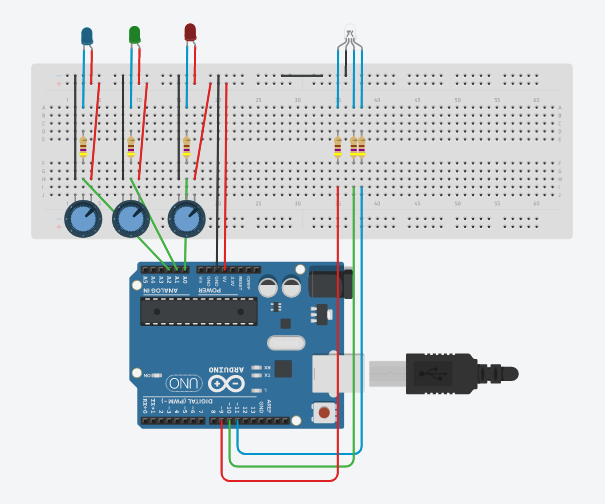
\includegraphics[scale = 0.6]{Figures/light-color-comb.png}
    \caption{Circuit diagram}
\end{figure}

\subsection*{Procedure}
\begin{enumerate}[leftmargin=*]
    \item Copy lst. \ref{lst:rgb} to a new Arduino sketchbook. Upload the code to your Arduino board.
    \item Rotate the knobs of the potentiometers to change the intensity of each primary color and observe the changes in all four LEDs.
\end{enumerate}

\begin{lstlisting}[language=Arduino, numbers=none, caption={Arduino code for measuring and calibrating the intensity of light in the LEDs}, captionpos=b, label={lst:rgb}]


int red   = A0;
int green = A1;
int blue  = A2;

int r=9, g=10, b=11;
int r1,g1,b1;

void setup() 
{
  // put your setup code here, to run once:
  
  // Input peripherals
  pinMode(red, INPUT);  
  pinMode(green, INPUT);  
  pinMode(blue, INPUT); 
  
  // Output peripherals
  pinMode(r, OUTPUT);  
  pinMode(g, OUTPUT);
  pinMode(b, OUTPUT);  
  
  Serial.begin(9600);
}

void loop() 
{
  // put your main code here, to run repeatedly:
  
  int red_intensity = analogRead(red);  
  int green_intensity = analogRead(green); 
  int blue_intensity = analogRead(blue); 
  // The intensity of light on the red, green and blue LEDs is recorded
  
  Serial.println(red_intensity*100/1024);   
  Serial.print("\t");
  Serial.print(green_intensity*100/1024);  
  Serial.print("\t");
  Serial.print(blue_intensity*100/1024);  
  // The light intensity is printed on Serial Monitor

  r1 = map(red_intensity, 0, 1023, 0, 255);
  g1 = map(green_intensity, 0, 1023, 0, 255);
  b1 = map(blue_intensity, 0, 1023, 0, 255);
  analogWrite(r, r1);
  analogWrite(g, g1);
  analogWrite(b, b1);
  // The red, green and blue LEDs of the RGB LED glow with  the same intensity as the red, blue and green LEDs controlled by the potentiometer.
}

\end{lstlisting}

\begin{figure}[H]
    \centering
    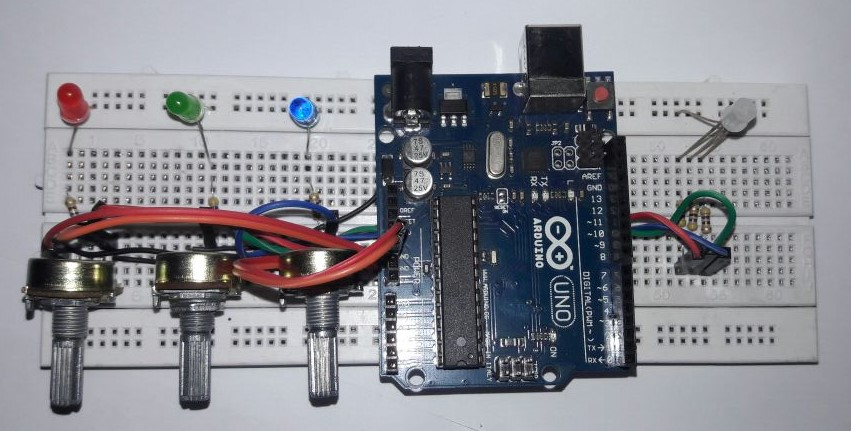
\includegraphics[scale = 0.5]{Figures/formation-of-colors.jpg}
    \caption{Hardware of the experiment}
\end{figure}
% --------------------------------------------------

\section*{3. Variation in the intensity of light with the change in medium}

For this experiment, you will need:
\begin{table}[H]
    \centering
    \begin{tabular}{|c|l|c|}\hline
     \textbf{\#} & \textbf{Components} &  \textbf{Amount}\\\hline
    1 & LDR                 & 1\\\hline
    2 & Torch               & 1\\ \hline
    3 & Arduino UNO       & 1 \\\hline
    4 & Breadboard          & 1 \\\hline
    5 & Connecting wires    & - \\\hline
    \end{tabular}
\end{table}

\subsubsection*{Connections}
\begin{enumerate}[leftmargin=*]
    \item Connect the 5V pin and GND pin of the Arduino board on the breadboard. 
    \item Connect one terminal of the LDR to 5V.
    \item Connect one terminal of the 1 k$\Omega$ resistor to the free terminal of the LDR. Connect its other terminal to GND.
    \item Connect the junction of the LDR and the resistor to pin A$0$ of the Arduino board.
    \item Connect the cathode of the LED to GND through a 470 $\Omega$ resistor. Connect its anode to pin 9 of Arduino.
\end{enumerate}

\begin{figure}[H]
    \centering
    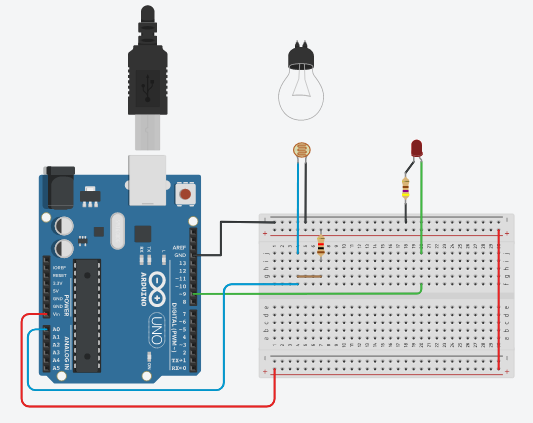
\includegraphics[scale=0.6]{Figures/light-transmission}
    \caption{Circuit diagram}
    \label{fig:my_label}
\end{figure}

\subsubsection*{Procedure}
\begin{enumerate}[leftmargin=*]
    \item Copy lst. \ref{lst:intensity} to a new Arduino sketchbook. Upload the code to your Arduino board. Also open the Serial Monitor or Serial Plotter.
    \item Shine a bright light on the LDR. Observe the change in the readings taken by Arduino.
    \item Place a transparent object between the LDR and the source of light. Observe the change in the readings taken by Arduino.
    \item Repeat the experiment with other types of objects (translucent and opaque) and note the difference in the intensity of light in each case.
\end{enumerate}
%Arduino Code
\begin{lstlisting}[language=Arduino, numbers=none, caption={Arduino code for measuring the intensity of light detected by LDR}, captionpos=b, label={lst:intensity}]

int shadow=A0;  
int led=9;

void setup() 
{
      // put your setup code here, to run once:
      pinMode(shadow, INPUT);   // A0 is declared an input peripheral
      pinMode (led, OUTPUT);     // Pin 9 is declared an output peripheral
      Serial.begin(9600);
}

void loop() 
{
      // put your main code here, to run repeatedly:
      
      int intensity = analogRead(shadow);    
      // The intensity of light on the LDR is recorded
      
      Serial.println(intensity);          
      // The light intensity is printed either on Serial Monitor or on Serial Plotter
      
      analogWrite(led, intensity/4);    
            
      delay(50);                      //Add a delay of 50 ms
}

\end{lstlisting}